\documentclass[onecolumn,nofootinbib,longbibliography,preprintnumbers,amsmath,amssymb,authblk,10pt]{revtex4-2}
\usepackage{amsmath,amssymb, tabularx,booktabs,physics,verbatim,soul,xcolor,tikz}
\usetikzlibrary{shapes, positioning, calc, arrows}

\newcommand{\drawCirclePair}[7]{
	\draw (#1,#2) circle (#4);
	\node at (#1,#2) {#5};
	
	\draw (#1+#3,#2) circle (#4);
	\node at (#1+#3,#2) {#6}; \draw[#7] (#1+#4, #2) -- (#1+#3-#4, #2); }

\newcommand{\drawCircle}[4]{
	\draw (#1,#2) circle (#4);
	\node at (#1,#2) {#3};
}

\begin{document}

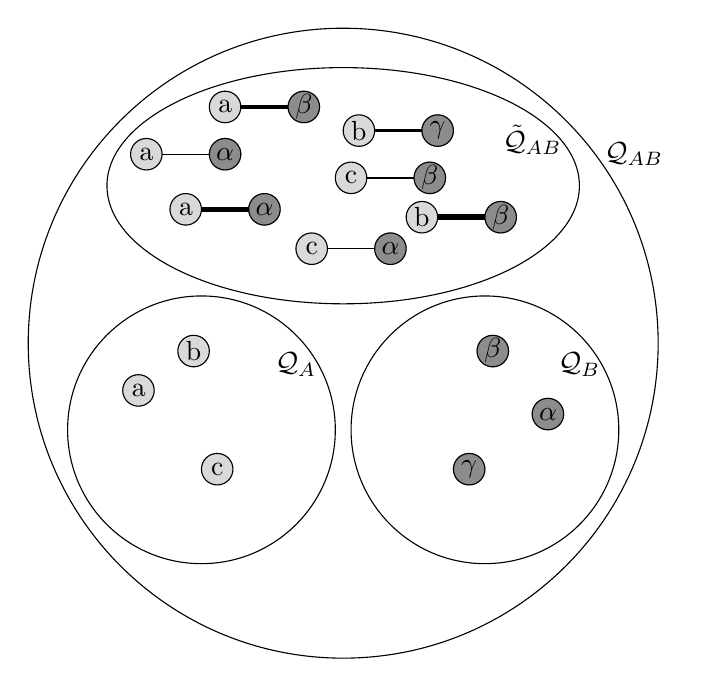
\begin{tikzpicture}
	\draw (0,0) ellipse (3 and 1.5);
	\filldraw[gray!30] (-2.5, 0.4) circle (0.2);
	\filldraw[gray!90] (-1.5, 0.4) circle (0.2);
	\drawCirclePair{-2.5}{0.4}{1}{0.2}{a}{$\alpha$}{line width=0.1mm}
	\filldraw[gray!30] (-2, -0.3) circle (0.2);
	\filldraw[gray!90] (-1, -0.3) circle (0.2);
	\drawCirclePair{-2}{-0.3}{1}{0.2}{a}{$\alpha$}{line width=0.7mm}
	\filldraw[gray!30] (-1.5, 1) circle (0.2);
	\filldraw[gray!90] (-0.5, 1) circle (0.2);
	\drawCirclePair{-1.5}{1}{1}{0.2}{a}{$\beta$}{line width=0.6mm}
	\filldraw[gray!30] (0.2,0.7) circle (0.2);
	\filldraw[gray!90] (1.2,0.7) circle (0.2);
	\drawCirclePair{0.2}{0.7}{1}{0.2}{b}{$\gamma$}{line width=0.4mm}
	\filldraw[gray!30] (0.1,0.1) circle (0.2);
	\filldraw[gray!90] (1.1,0.1) circle (0.2);
	\drawCirclePair{0.1}{0.1}{1}{0.2}{c}{$\beta$}{line width=0.3mm}
	\filldraw[gray!30] (-0.4,-0.8) circle (0.2);
	\filldraw[gray!90] (0.6,-0.8) circle (0.2);
	\drawCirclePair{-0.4}{-0.8}{1}{0.2}{c}{$\alpha$}{line width=0.2mm}
	\filldraw[gray!30] (1,-0.4) circle (0.2);
	\filldraw[gray!90] (2,-0.4) circle (0.2);
	\drawCirclePair{1}{-0.4}{1}{0.2}{b}{$\beta$}{line width=0.8mm}
	\node[below] at (2.4, 0.9) {$\tilde{\mathcal{Q}}_{AB}$};



	\draw (0, -2) circle (4);

	\draw (-1.8, -3.1) circle (1.7);
	\filldraw[gray!30] (-2.6,-2.6) circle (0.2);
	\filldraw[gray!30] (-1.9,-2.1) circle (0.2);
	\filldraw[gray!30] (-1.6,-3.6) circle (0.2);
	\drawCircle{-2.6}{-2.6}{a}{0.2}
	\drawCircle{-1.9}{-2.1}{b}{0.2}
	\drawCircle{-1.6}{-3.6}{c}{0.2}
	\node[below] at (-0.6, -2) {$\mathcal{Q}_A$};

	\draw (1.8, -3.1) circle (1.7);
	\filldraw[gray!90] (2.6,-2.9) circle (0.2);
	\filldraw[gray!90] (1.9,-2.1) circle (0.2);
	\filldraw[gray!90] (1.6,-3.6) circle (0.2);
	\drawCircle{2.6}{-2.9}{$\alpha$}{0.2}
	\drawCircle{1.9}{-2.1}{$\beta$}{0.2}
	\drawCircle{1.6}{-3.6}{$\gamma$}{0.2}
	\node[below] at (3.0, -2) {$\mathcal{Q}_B$};

	\node[right] at (3.2, 0.4) {$\mathcal{Q}_{AB}$};
\end{tikzpicture}

\end{document}